\documentclass[letterpaper,twocolumn,10pt]{article}
\usepackage{../usenix-2020-09}
\usepackage{../findlay}
\usepackage{enumitem}

% Silence annoying warning about nonfrench spacing
\microtypecontext{spacing=nonfrench}

% Enum with custom labels for design Goals
\newlist{dgenum}{enumerate}{1}
\setlist[dgenum]{label=\arabic*., ref=\arabic*}
\crefname{design goal}{Design Goal}{Design Goals}
\crefalias{dgenumi}{design goal}

%-------------------------------------------------------------------------------
\begin{document}
%-------------------------------------------------------------------------------

%don't want date printed
%\date{}

% make title bold and 14 pt font (Latex default is non-bold, 16 pt)
\title{\Large \bf Houdini: Security Benchmarking of Container Confinement}
%for single author (just remove % characters)
% TODO: Authors hidden for anonymous submission
% \author{
% {\rm William P\@. Findlay}\\
% Carleton University
% \and
% {\rm Kevin Guy}\\
% Carleton University
% \and
% {\rm David Barrera}\\
% Carleton University
% \and
% {\rm Anil Somayaji}\\
% Carleton University
% } % end author

\maketitle

\begin{abstract}
  While container-based workloads are now a standard part of our cloud infrastructure, container security remains a challenging problem.  Container confinement is a particularly pressing problem, as without it a single vulnerable application can be used to compromise entire clusters of containers.  While we have many technologies that can be used to secure containers, currently there is no easy way to determine whether a given configuration provides even a basic level of protection.  Here we present \houdini, a security benchmark for container confinement.  Much as network scanning tools can help catch misconfigured firewalls, \houdini can check whether a given container configuration properly enforces confinement.  While it can be used to test deployable containers, \houdini is optimised for testing and comparing container confinement technologies.  Here we present the motivation, design, implementation, and initial results on running \houdini on a set of privileged and unprivileged container configurations.  By providing a benchmark framework by which container confinement technologies can be evaluated, we believe \houdini can help foster the development of next-generation container confinement technologies.
\end{abstract}

\section{Introduction}

Container-based workloads have become a cornerstone of modern cloud infrastructure, which has revolutionized how applications are developed, deployed, and scaled. Unlike hypervisor-based virtual machines, which require a full operating system for each instance and rely on a hypervisor to manage hardware virtualization, containers are lightweight, share the host system’s kernel, and incur minimal overhead. This efficiency has made containers an attractive choice for organizations seeking to optimize resource utilization and reduce operational costs. Furthermore, containers enable seamless portability by encapsulating all userspace dependencies into a unified image. Despite container's numerous benefits, they introduce new security challenges, particularly around container confinement. Container confinement can be defined as the set of mechanisms and strategies used to isolate a containerized application from the host system and other containers. Effective confinement is critical for maintaining system security and stability, as it ensures that containers operate within defined boundaries by restricting their access to system resources, processes, and networks. 


Linux features such as cgroups, namespaces, and mountpoints create the appearance of isolation for containers. These mechanisms ensure that they are confined to their own resource, process, and network boundaries. However, this separation can fail due to kernel vulnerabilities, misconfigurations, or even sophisticated attacks like container escapes, allowing attackers to disrupt other containers or compromise the host system. Technologies like SELinux, AppArmor, and seccomp provide additional layers of security but are notoriously complex to configure and prone to misconfiguration. A best practices guide for container security  \cite{CIS} can help with configuring a container, but it offers no guarantee that the resulting configuration performs as intended. For instance, how can we confirm that cgroups and namespaces are restricting containers as intended? As container adoption skyrocketed across industries, particularly in multi-tenant cloud environments, these security challenges have become more pronounced. To address this challenge, the cloud industry has developed technologies like gVisor and Kata Containers, which isolate containers further by running them within lightweight virtual machines. While this approach is effective, it unnecessarily increases complexity and overhead. By developing methods to audit and validate confinement mechanisms, container security could be simplified by reducing reliance on such solutions.

Test suites play a crucial role in ensuring that systems meet requirements and function correctly under defined conditions. For instance, the SPEC (Standard Performance Evaluation Corporation) benchmarks measure CPU performance and power efficiency, while the TPC (Transaction Processing Performance Council) benchmarks assess database performance. The Phoronix Test Suite is another widely used option, particularly in Linux-based systems. Other notable benchmarks include Geekbench, a cross-platform tool for evaluating CPU and GPU performance, and IOzone, which focuses on file system I/O performance. In software development, regression tests play a critical role in ensuring that code changes do not inadvertently break existing functionality. Many organizations enforce policies requiring code to pass these tests before integration. Test suites also ensure the functionality of production systems, such as uptime monitors that verify whether services are operating as intended. Additionally, functional test suites, though less frequently used, help identify security vulnerabilities in deployed systems. Tools like network scanners are especially valuable for detecting misconfigurations, insecure software versions, and unintended service exposures.

Despite the widespread use of test suites in these areas, a significant gap remains in the context of containers. There are currently no standardized or widely adopted test suites designed specifically to evaluate container security, functionality, or isolation effectiveness. This absence leaves organizations relying on ad hoc methods, which are often inadequate for uncovering subtle vulnerabilities or ensuring robust confinement. Given the growing reliance on containerized environments in modern infrastructure, the development of comprehensive test suites tailored for containers is imperative. Such test suites would not only address these critical gaps but also provide a reliable foundation for improving trust and security in containerized systems.

In this paper, we describe the implementation of \houdini, the first test suite for verifying container confinement. Given a Docker container configuration (including both the kernel version and the docker version), Houdini will instantiate the container in a standalone QEMU-based virtual machine and perform multiple tests (or tricks, as we call them) to evaluate whether the configuration is susceptible to various forms of container misconfigurations or failures. These tests explore vulnerabilities that could disrupt container functionality, such as improper resource allocation, inadequate isolation, or insecure filesystem setups. Houdini is written in Python and is easily extensible, providing an extension language for writing tricks. Houdini is designed to assess and enhance the security of containerized environments. It tests the isolation of containers, ensuring they remain properly confined and separated from the host system and other containers. Houdini specializes in identifying container-specific vulnerabilities, misconfigurations, and ensuring adherence to security best practices.

A standard methodology for assessing container confinement is crucial due to the complexity of modern systems and the intricate vulnerabilities they present. A formal approach involving the rigorously evaluating and analyzing the security of the container system might seem ideal, however, it is impractical because container environments are highly complex, with interactions between kernels, runtimes, orchestration tools, and external dependencies that are difficult to model comprehensively. Moreover, many vulnerabilities stem from subtle details that a formal model might overlook. Instead, an empirical approach offers a practical alternative. Though it will never be exhaustive, the goal is not comprehensive coverage but rather establishing a baseline set of tests that demonstrate effective container confinement. This approach is achievable and can evolve over time as new vulnerabilities are identified, allowing the methodology to remain current. Starting with tests for isolation, privilege escalation prevention, resource limitation enforcement, and resistance to known exploits provides a solid foundation. By focusing on demonstrating security effectiveness in critical areas, this methodology can enhance confidence in container confinement while enabling continuous improvement and adaptation to the evolving threat landscape.

In this paper we describe Houdini's motivation, design, and implementation. We also present the results of case studies showing how Houdini can be used to detect misconfigured containers that allow for privilege escalation attacks on the host system. Our hope with Houdini is that it will help with the deployment of better confined containers and will support the development of new technologies to more reliably confine containers.

The rest of this paper proceeds as follows. In Section~\ref{sec:confinement}, we explain the container confinement problem and associated technologies.  We describe Houdini's design and implementation in Section~\ref{sec:design}. Section~\ref{sec:testing-confinement} explains the tricks Houdini currently implements and their associated vulnerabilities.  In Section~\ref{sec:evaluation} we present case studies showing how Houdini can detect basic misconfigurations.  Section~\ref{sec:related} describes related work, Section~\ref{sec:discussion} discusses the contributions, limitations, and our plans for future work.  Section~\ref{sec:conclusion} concludes our paper.


%% While containers are widely used, despite their name they don't currently offer strong confinement guarantees. Numerous ways for procesess inside a container to "escape".  While originally containers were designed for administration and software distribution purposes, there is increasing interest in improving container confinement.

%% Variety of solutions:
%% \begin{itemize}
%% \item host-based security mechanisms applied to enforce confinement on processes inside containers (SELinux, AppArmor, system call filters)
%% \item hardware virtualization applied to container confinement (gVisor, kata containers - also known as microVMs, )
%% \item new kernel-level security abstractions, often implemented in eBPF (bpfbox, bpfcontain on archive)
%% \end{itemize}

%% Our question: how effective are these container confinement solutions?

%% Needed: a standard methodology for assessing container confinement
%% \begin{itemize}
%% \item formal approach not feasible, systems are too complex and vulnerabilities are in the details
%% \item empirical approach is possible.  Will never be comprehensive, but that is not the goal.  Instead, we want a baseline set of tests (that can be improved over time) that demonstrates effective container confinement.
%% \end{itemize}

%% Contribution: Houdini, first tool for automated testing of container confinement
%% \begin{itemize}
%% \item series of tests for well-known container vulnerabilities
%% \item designed to facilitate repeatable experiments using qemu-based virtual machines
%% \item easily extensible to allow for new tests to be added, making Houdini more comprehensive over time
%% \end{itemize}
%% (NOTE: we should specify how to "version" Houdini so we can talk about both older and newer versions of Houdini.  So we don't just want a Houdini score, it should be a versioned Houdini score.)

\section{Container Confinement Problem}
\label{sec:confinement}

Container confinement can be defined as the set of mechanisms and strategies used to isolate a containerized application from the host system and other containers. Effective confinement is critical for maintaining system security and stability, as it ensures that containers operate within defined boundaries by restricting their access to system resources, processes, and networks. 

The level of confinement of a container is not fixed; it can vary based on the specific requirements or intentions of the user. In other words, the degree to which a container is isolated from the host system or other containers is customizable to meet the user’s needs. The optimal configuration, however, is one that strikes a balance between maximum confinement (restricting access to system resources as much as possible) and functional flexibility (enabling the container to perform its intended tasks). Achieving this balance is the core goal of container confinement. 


There is a semantic gap in containerized systems, where the intended security policies and the actual behavior of the system don't always align. The semantic gap refers to the difference between what a system is meant to do and how it actually behaves in practice. In other words, it’s the disconnect between the theoretical design of the system and its real-world execution. This gap can occur for various reasons, such as miscommunications, misunderstandings, or limitations in the system's design or configuration.

For example, when setting up a security system, an administrator may want to ensure that containers in a cloud environment are completely isolated from each other and the host system. The goal is to set up strict access controls so that containers cannot interact with each other or the host. However, due to complex settings, misconfigurations, or flaws in how security mechanisms (like namespaces, cgroups, SELinux, etc.) interact, the system might not enforce these isolation policies correctly. As a result, the actual performance may not align with the intended security model.

This gap can happen in many systems, but it is especially common in complex environments like containers, where multiple interdependent components (e.g., the container runtime, kernel features, and security tools) must work together smoothly. Misunderstandings or mistakes in configuring these components can lead to unexpected issues or security vulnerabilities, even when the system seems correctly set up. The semantic gap highlights the challenge of ensuring that the real-world behavior of the system matches the user’s or designer’s intentions. Houdini helps bridge this gap in container confinement by providing an empirical framework to test and verify whether a container’s security mechanisms are functioning as intended.




% Since the process of setting up effective container confinement involves balancing maximum isolation with the functional flexibility that allows the container to perform its intended tasks, Houdini provides a mechanism for continuous testing and refinement to reach that balance. In other words, \houdini lets you confine a container by allowing users to iterate and fine-tune the container’s security settings until they achieve an optimal level of confinement.
\section{Design and Implementation}
\label{sec:design}

\subsection{Design Goals}

With the creation of \houdini, we sought to rectify a critical perceived gap in existing
security testing frameworks. In particular, we noticed that no existing testing framework
satisfied our specific use case: testing the isolation guarantees of a research artifact
in a highly reproducible manner, independent of the underlying container runtime and the
implementation details of the enforcement mechanism. (Refer to \Cref{sec:related} for
a detailed comparison with existing work on container security evaluation.)

In order to achieve the aforementioned result, we designed \houdini with the following
goals in mind:
\begin{dgenum}
  \item \label{dg:repro}\textit{Reproducible Results.} Results of a test should be
  reproducible over time and across various system configurations. Reproducibility is
  a critical property of the scientific method and quintessential to the integrity of
  academic research evaluations. Our hope is that reproducible security evaluations will
  promote the use of \houdini to enable fair and unbiased comparisons of container security
  artifacts based on their security properties.

  \item \label{dg:platform}\textit{Controlled Environment.} \houdini should be capable of
  evaluating a security artifact independently of the underlying platform (e.g\@. the
  container runtime, host operating system, and whatever security measures are in place,
  if any). Platform independence helps to ensure that the focus of a security evaluation
  is on the effectiveness of whatever protections are being tested as opposed to
  differences in the underlying platform (e.g\@. bugs, configuration differences, or
  version specific behaviors).

  \item \label{dg:container}\textit{Container Specificity.} While a number of security
  testing frameworks exist, very few target the container specific use case we want to
  support with \houdini: container security. This motivated us to consider an
  implementation which focuses specifically on the container security use case.

  \item \label{dg:flex}\textit{Test Case Expressiveness.} \houdini test cases (called
  \enquote{tricks}) should be maximally expressive, such that some combination of steps
  can be used to achieve and test any desired result. It should be possible to define
  a new \houdini trick and modify existing tricks without modifying the \houdini
  binary. Moreover, it should be clear from reading a defined trick precisely what steps
  are involved, the consequences of each step passing or failing, and the overall nature
  of the exploit being tested.
\end{dgenum}

We wrote \houdini in just over 3300 lines of Rust code\footnote{Source lines of code,
i.e\@. not counting whitespace, comments, and dependencies.}. Rust offers several
desirable properties for a security benchmarking application like \houdini. First, Rust
has a rich ecosystem of libraries (called \enquote{crates}) that enable us to easily work
with external APIs such as the Docker daemon. Moreover, Rust has excellent support for
serializing and deserializing YAML and JSON to and from Rust enums and data structures using
powerful macros exposed by the \texttt{serde} crate. Finally, Rust's \texttt{tokio} crate
provides a powerful asynchronous framework that enables us to easily parallelize and
synchronize \houdini tricks and their steps.

\todo{talk about security and how we shouldn't need to worry about the tricks being used
maliciously (we're testing armour and brining our own weapons and test range, we're not
really worried terrorists coming in and blowing us up)}

\subsection{Houdini Tricks}

Exploits that \houdini can test are broken up into individual files called
\textit{tricks} (\Cref{dg:flex}). Each \houdini trick is written in YAML and consists of a metadata section
followed by one or more \textit{steps}. \houdini comes with a stock set of tricks (c.f\@.
\Cref{sec:testing-confinement}), tested in continuous integration to ensure they always
work by default under vulnerable configurations.

While these default tricks can provide decent exploit coverage for initial tests, it is
also possible for the user to write their own tricks by defining their own YAML files
following the expected format. This modular design enables \houdini to test essentially
any container escape while providing the ability for the user to modify existing tricks
should the need arise (e.g\@. to test a specific aspect of a defense mechanism in a more
targeted fashion).

\Cref{lst:mounted-docker-socket} provides a simple example of a \houdini trick that tests
whether a mounted Docker socket in a container can be used to communicate with the Docker
daemon running on the host. Steps in a \houdini trick consist of an ordered list of
parameterized, well-defined actions. In our current implementation, there are six distinct
types of step:

\begin{itemize}
  \item \texttt{VersionCheck} enforces a version check on the host operating system version,
  docker daemon version, and container runtime version (e.g\@. \texttt{runc}). This helps
  to verify that a trick is indeed running under an expected configuration where it
  would ordinarily succeed without any additional protections in place.

  \item \texttt{SpawnContainer}

  \item \texttt{KillContainer}

  \item \texttt{Host}

  \item \texttt{Container}

  \item \texttt{Wait}
\end{itemize}

\begin{listing}
  \caption{A YAML definition of a Houdini trick with three steps. The first step spawns
  a container from the \enquote{bash} Docker image, downloading it if necessary. As part
  of the exploit setup, we mount \texttt{/var/run/docker.sock} from the host into the
  container. The second step installs curl into the bash container. Finally, the third
  step attempts to abuse the mounted Docker socket to make API requests to Docker. Note the
  status codes on success and failure for each step in the Trick.}
  \label{lst:mounted-docker-socket}
  \begin{minted}[frame=lines,framesep=2mm]{yaml}
  name: mounted-docker-socket
  steps:
    - spawnContainer:
        name: bash
        image: bash
        cmd: sleep infinity
        volumes:
        - "/var/run/docker.sock:/docker.sock"
        failure: setupFailure
    - container:
        name: bash
        script:
        - command: apk
          args:
          - add
          - curl
        failure: setupFailure
    - container:
        name: bash
        script:
        - command: curl
          args:
          - "--unix-socket"
          - "/docker.sock"
          - "http://localhost/_ping"
        failure: exploitFailure
        success: exploitSuccess
  \end{minted}
\end{listing}

\subsection{Reproducible Tricks}

\todo{WILLIAM: Houdini design and implementation details here.}


\begin{figure}
  \label{fig:state-machine}
  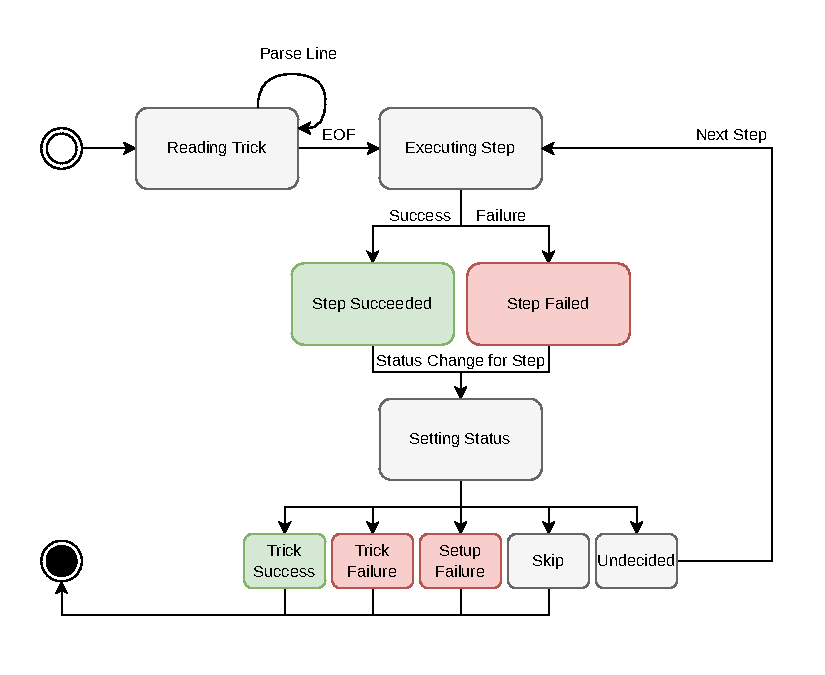
\includegraphics[width=1\linewidth]{figs/houdini-state-machine.pdf}
  \caption{A state machine diagram of Houdini running a Trick. Note that aside from the
  \enquote{Undecided} status, all other statuses are considered final. That is, a step
  reporting such a status terminates execution of the Trick.}
\end{figure}

\todo{WILLIAM: Introduce the architecture diagram below somehow (what is the best way to do this?)}

\begin{itemize}
\item security problems arise from vuln in specific components
\item if we're going to be testing, we need to have an idea of what components we're testing
\item ideal coverage will touch everything
\item some components are targeted more frequently than others in attacks commonly used in practice
\end{itemize}

\begin{figure}
  \label{fig:architecture}
  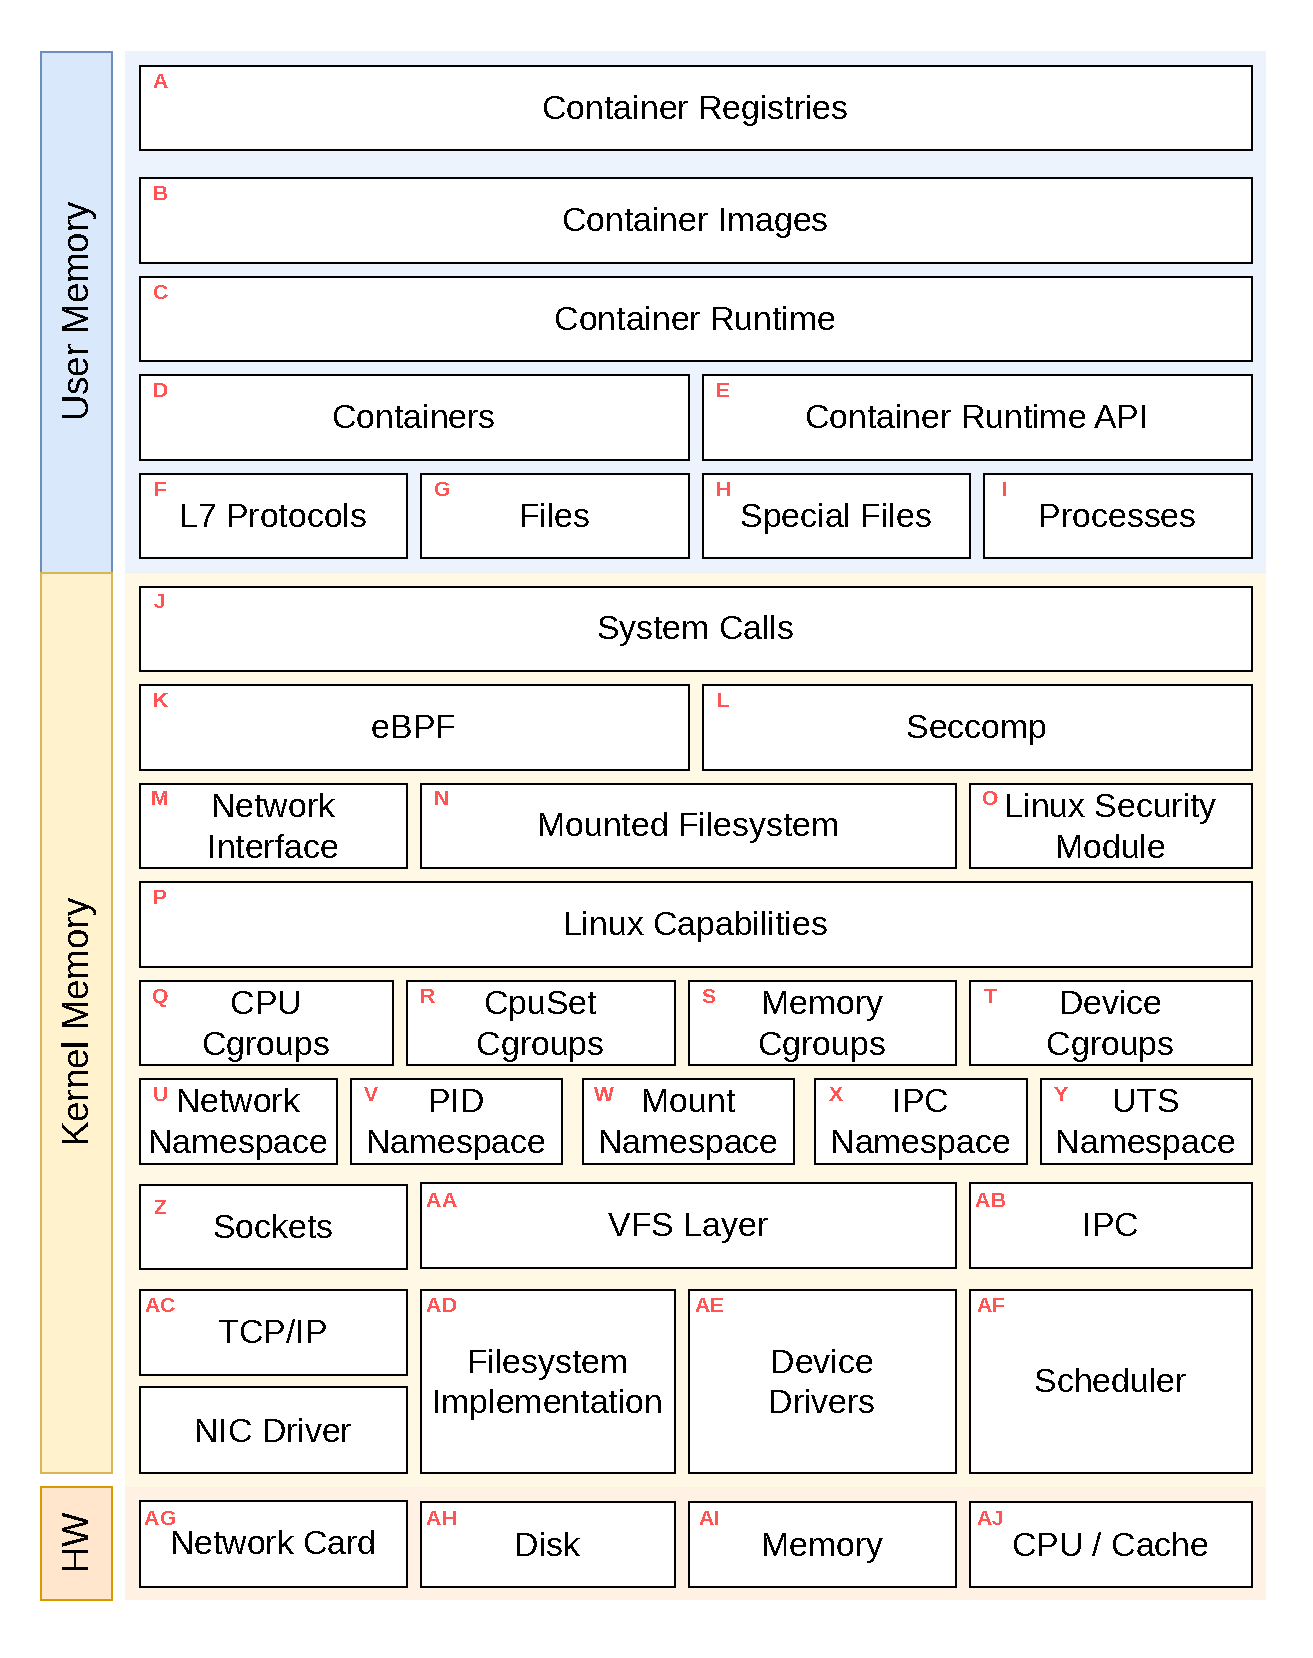
\includegraphics[width=1\linewidth]{figs/exploit-coverage.pdf}
  \caption{An architectural diagram of a container deployment environment depicting the
  attack surface created by its various components. Components are organized
  hierarchically with lower level subsystems toward the bottom, including data structures
  and abstractions that reside in kernel memory and the hardware itself.}
\end{figure}

\section{Testing Confinement}
\label{sec:testing-confinement}

\begin{table*}
  \caption{\todo{table caption}}
  \label{tab:classification}
  \centering \small
  \begin{tabular}{lllll}
    \toprule
    \bfseries No\@. & \bfseries Exploit & & \bfseries CVE No\@. & \bfseries Attack Vectors \normalfont{(See \Cref{fig:architecture})} \\
    \midrule
    1 & Mounted Docker Socket               & CITE & ---            & C, D, E, N \\
    2 & Mounted \texttt{/etc/passwd}        & CITE & ---            & C, D, G, K \\
    3 & Pipes Read-Only Overwrite           & CITE & CVE-2022-0847  & O, S \\
    4 & Cgroup Release Agent Code Execution & CITE & CVE-2022-0492  & M, O, R \\
    5 & Apache Path Traversal               & CITE & CVE-2021-42013 & D, I \\
    6 & \texttt{runc} Binary Overwrite      & CITE & CVE-2019-5736  & A, B, C, D, H, K \\
    \bottomrule
  \end{tabular}
\end{table*}

\todo{KEVIN: Explain some technical details for each exploit. Refer back to \Cref{tab:classification} as necessary.}

% https://unit42.paloaltonetworks.com/breaking-docker-via-runc-explaining-cve-2019-5736/
% https://nvd.nist.gov/vuln/detail/CVE-2019-5736
% exploits the container runtime runc [C, E?], the procfs filesystem [H, K], process IDs [P]
% RCE, elevation of privilege, DoS
\noindent\textbf{CVE-2019-5736.} This CVE\cite{addtheref} is a remote code execution vulnerability in the \texttt{runc} binary. The PoC exploits the way \texttt{runc} creates a process in the container called \texttt{runcInit} to run a specified command. The \texttt{procfs} file system contains a symlink to the binary being executed in \texttt{/proc/self/exe} which points to the \texttt{runc} executable on the host. A malicious container overwrites its own \texttt{/bin/sh} binary to the \texttt{/proc/self/exe} interpreter \texttt{\#!/proc/self/exe}. Once a user executes the overwritten \texttt{/bin/sh} binary, the interpreter calls the \texttt{runc} binary whose pid is then captured. Malicious code will then obtain the file descriptor from \texttt{/proc/runc-pid/exe} and overwrite the contents of the \texttt{runc} binary on the host.

% https://blog.qualys.com/vulnerabilities-threat-research/2021/10/27/apache-http-server-path-traversal-remote-code-execution-cve-2021-41773-cve-2021-42013
% https://nvd.nist.gov/vuln/detail/CVE-2021-42013
% exploits a specific vulnerable application in the container [D] through HTTP urls containing file traversal character sequences
% RCE
\noindent\textbf{CVE-2021-42013.} This is a remote code execution vulnerability in the Apache HTTP server container (versions 2.4.49 and 2.4.50). The exploit is a path traversal vulnerability that takes advantage of the server being unable to detect the path traversal characters ``../'' in a URL. This may occur when the second dot is replaced by its unicode representation ``\%2e''. By requesting a URL with several path traversal sequences and a binary to execute, contents of files can be retrieved from the container's local filesystem.

% https://dirtypipe.cm4all.com/
% https://nvd.nist.gov/vuln/detail/CVE-2022-0492
% exploits the cgroup file system [K, R?], cgroups [M], processes [I], special files that interact with the cgroups [H?], the way container filesystems are stored on the host [O, R?]
% RCE, elevation of privilege, information disclosure
\noindent\textbf{CVE-2022-0492.} A bug in the kernel's \detokenize{cgroup_release_agent_write cgroupv1} filesystem code can be exploited to enable a container escape. A file called \detokenize{release_agent} gets executed when a process in the cgroup terminates if \detokenize{notify_on_release} is enabled. The exploit involves mounting the cgroups filesystem on the host to the container and creating a directory which creates a new cgroup. Creating the \detokenize{notify_on_release} file in the new directory and writing a 1 to it tells the host to run the \detokenize{release_agent} file when a process in the custom cgroup terminates. Modifying the \detokenize{release_agent} file with a script that executes a malicious binary on the container from the host's filesystem allows the malicious container to successfully escape upon termination of a process in the custom cgroup.

% https://sysdig.com/blog/detecting-mitigating-cve-2022-0492-sysdig/
% https://nvd.nist.gov/vuln/detail/CVE-2022-0847
% exploits a vulnerability in the pipe.c code [S] that allows data within a spliced page cache to be overwritten if pipe is set up in a specific way
% RCE, elevation of privilege, DoS
\noindent\textbf{CVE-2022-0847.} This is an escalation of privilege Linux kernel vulnerability caused by a bug in the kernel's pipe.c code introduced in version 5.8. The exploit utilizes the pipe buffers flag \detokenize{PIPE_BUF_FLAG_CAN_MERGE} which allows for data to be overwritten in a page cache from a spliced file if the pipe buffer is prepared in a specific way. The flag gets set by filling the buffer with random data. The pipe buffer can then be emptied and then a file can be spliced into the pipe. Writing data into the pipe buffer now overwrites the data in the file. In order to escape a container with this exploit, the setup is similar to that of CVE-2019-5736 above where a malicious container waits for runc to execute in the container. The file descriptor is grabbed from the procfs and overwritten using the dirty pipe vulnerability.

We selected the exploits above based on several criteria. (1) The exploits must have a proof of concept readily available online; (2) the exploits must cover various components of the container deployment environment (see \Cref{fig:architecture}); and (3) the exploits must be high impact and severity defined by the CVS standards. The exploits chosen all fit within these criteria and can be tested repeatedly with different system configurations using \houdini.

The exploits are run in privileged and unprivileged mode with one of seccomp or apparmor securing the container. Most exploits are blocked successfully by using these security systems, but these security systems might not be configured or enabled by default. For example, kernels can come with apparmor on the system but it is disabled by default on boot and the service must be re-enabled by manipulating GRUB boot parameters. Using Docker info on a system lets a user know what container security mechanisms are available to the user. If apparmor is not installed on the system or the service is not enabled on boot through GRUB, then seccomp is usually the only security mechanism that can be deployed.

The default policy files for both apparmor and seccomp are used during testing. The default policy for apparmor most importantly restricts write permissions in the sensitive \texttt{/proc} and \texttt{/sys} file sysytems, as well as denying mounting operations. The default seccomp profile allows for all but 44 of the system calls to pass through and can allow more based on the container's capabilities. The system calls that are filtered out and restricted are focused around sensitive operations that can interact directly with the host kernel and potentially modify its behaviour (kernel modules, system time, reboot, etc.).

Tests were run on Ubuntu 22.04 with kernel version 5.15.0-50-generic. The docker engine is version 18.09.1 and runc version is 1.1.0+dev. For virtualization we used QEMU version 6.2.0 and buildroot version 2022.02.

We manually created a trick yaml file for each exploit outlining the environment and the commands for the host and container to perform. If required for the exploit, a new environment is created using the buildroot to generate a new virtual machine with a configurable linux kernel and filesystem. The versions for the kernel and specific packages that are required to run the exploit successfully, such as docker and runc, that are specified in the exploit yaml are passed to buildroot as parameters. Houdini is also included as a package and launches when the virtual system boots. QEMU runs the virtual environment and creates a virtual socket (vsock) connection between the host and the VM for status reporting and management. Once \houdini on the VM boots, a connection is made to \houdini running on the host. The trick is then sent via the vsock connection and parsed by the \houdini client on the VM and for the remainder of the trick, the VM is acting as the host. Once the trick finishes execution, the results are sent back to the host \houdini using the vsock connection and the VM is shut down.

The exploit CVE-2019-5736 is set up with a malicious container that runs a script on start to wait for the /bin/sh binary to execute and then in turn execute its own binary to overwrite the host runc. The vulnerable runc version being tested is version 1.0.0-rc6. On the host side, the user spins up the container and attempts to exec into the container using "docker exec -it ID sh". The exploit is considered a success if the runc binary on the host system has been compromised.

CVE-2021-42013 has a different threat model where the container image is vulnerable but not necessarily malicious. The exploit begins with a vulnerable apache httpd image being launched and then on the host side, the exploit binary is called using the container's IP address and a command as input. The exploit is considered a success if the command runs and data is received containing the response from the container.

Unlike the previous two exploits, CVE-2022-0492 does not utilize any malicious binaries. The exploit takes place with commands executed entirely within the container. A privileged container is launched and the cgroup rdma folder from the host cgroup filesystem is mounted in the container allowing for manipulation of the cgroup's release agent file. The exploit is considered successful if all commands execute successfully with no errors.

%%%%%%%%%%%%%%%%%%%% CVE-2022-0492 %%%%%%%%%%%%%%%%%%%%%%
% mkdir /tmp/mountest
% mount -t cgroup -o rdma cgroup /tmp/mountest
% mkdir /tmp/mountest/x
% echo 1 > /tmp/mountest/x/notify_on_release
% host_path=`sed -n 's/.*\perdir=\([^,]*\).*/\1/p' /etc/mtab`
% echo "$host_path/cmd" > /tmp/mountest/release_agent
% echo '#!/bin/sh' > /cmd
% echo "cat /etc/passwd > $host_path/output" >> /cmd
% chmod a+x /cmd
% sh -c "echo \$\$ > /tmp/mountest/x/cgroup.procs"
% cat /output

% display and explain results and how each test was ran

\begin{table*}
 \caption{\todo{table caption, replace success/failure text with glyphs. re-order, grouping unprivileged rows and privileged rows. }}
 \label{tab:results}
 \centering \small
 \begin{tabular}{lllll}
   \toprule
   \bfseries Security & \bfseries CVE-2019-5736 & \bfseries CVE-2021-42013 & \bfseries CVE-2022-0492 & \bfseries CVE-2022-0847 \normalfont{(See \Cref{fig:architecture})} \\
   \midrule
   unprivileged & success & success & failure & success \\
   privileged  & success & success & success & success \\
   unprivileged + apparmor & failure & success & failure & failure \\
   privileged + apparmor & failure & success & failure & failure\\
   unprivileged + seccomp & failure & success & failure & success\\
   privileged + seccomp & success & success &  success & success \\
   \bottomrule
 \end{tabular}
\end{table*}

\noindent\textbf{Why use Houdini.}

Container hardening techniques through confinement mechanisms require both knowledge of the application code and security best practices. Ensuring that their container environment is not vulnerable to known common exploits is a step that many developers will either save for the last part of their development cycle or forget about all together. Testing frameworks allow developers to save time by automatically running a suite of some tests in order to give the developer more insight into how their application behaves. Existing exploit testing frameworks are not designed with the goal of exposing problematic areas in a container's confinement policy or environment. \houdini allows the user to run a series of known vulnerabilities against their container environment to expose issues for the developer to quickly asses and act upon. The security mechanisms that are used to lockdown the container can easily be tested repeatedly throughout the development lifecycle without much overhead for the developer. \houdini also allows for the testing of new confinement mechanisms by academics and researchers with very little required customization to the trick files themselves. \houdini can test any part of the system for vulnerabilities including the kernel, runtime, and the container configuration which all contribute towards making the container vulnerable. This makes \houdini a powerful tool when assisting in the development of container confinement policies and environment testing.

\noindent\textbf{What makes running the exploit possible in apparmor.}

Apparmor and seccomp are integrated with docker to allow a user to further confine their resources and capabilities. When apparmor is enabled on a host kernel, docker will apply a default apparmor policy to a container. The policy name is docker default and it restricts: mounting, most cases of writing to /proc, and most cases of writing to /sys. This rather limited profile does a relatively good job of blocking common container escapes and privilege escalations. Issues mainly arise when a user tries to modify the existing policy, or develop their own without proper consideration. An apparmor profile is developed by specifying resources to allow or deny access to on each line. The profile must then be ran through the apparmor parser which checks for the proper syntax to be followed. Once the parser successfully reads and loads the profile, docker can use it as a value passed to their \detokenize{"--security-opts apparmor=PROFILE_NAME"} flag.

The apparmor parser will not check for whether a specified system path exists or not and if contradictory statements exist, it uses the statement that is more restrictive (i.e. if "mount" and "deny mount" exist in the same profile, it will always use "deny mount" no matter the declared order).

In order for CVE-2022-0492 to successfully operate with the apparmor security enabled on a privileged container, the only line that needs to be modified in the default profile is "deny mount". If a user were to change the "deny mount" to "mount" for either their own usage or as a simple mistake, then the exploit would be able to run successfully.

CVE-2019-5736 requires a little more modification to the docker default profile. Write access to \texttt{/proc/PID} must be allowed and full use of ptrace must be allowed. The exploit can successfully overwrite its own shell binary without any modifications to the default profile. If only write access to \texttt{/proc/PID} is given, the exploit can grab a hold of the runc process ID, but access to ptrace is required as it is used for process control by the system when modifying the \texttt{/proc/PID/exe} file. These two changes to the default apparmor profile allow CVE-2022-0492 to successfully overwrite the runc binary even without the privileged flag.

Using older versions of the container runtime RunC before version 1.0.0-rc8 allows for a different bypass of the apparmor confinement policy. Since apparmor is based off of path names, a malicious user can get around the default apparmor's policy that is locking down a specific path name by simply remounting it to a different path. An example of this is the procfs filesystem mounted on \texttt{/proc}. The Apparmor default profile locks down the procfs filesystem at the defined \texttt{/proc} location. By remounting the procfs filesystem to a different location, this bypasses the pathname based confinement that apparmor offers.

\noindent\textbf{What do the results tell us.}

\todo{docker default security profiles can be overly permissive. Why?}
\todo{seccomp by default allows almost 90\% of systemcalls}
\todo{apparmor allows all network capability}
\todo{default profiles are needed to be generic and more likely overly permissive}
\todo{generally do a good job catching existing exploits by locking down key parts}
\todo{Compromise between security and usability}
\todo{developing profiles can be difficult even with tools such as aa-easyprof}
\todo{testing confinement is made easy}


%%%%%%%%%%%%%%%%%%%%%%%%%%%% DEFAULT %%%%%%%%%%%%%%%%%%%%%%%%%%%%%%%%%%
% include <tunables/global>
%
% profile docker-default flags=(attach_disconnected,mediate_deleted) {
%
%   #include <abstractions/base>
%
%   ptrace peer=@{profile_name},
%
%   network,
%   capability,
%   file,
%   umount,
%
%   deny @{PROC}/* w,  # deny write for all files directly in /proc (not in a subdir)
%   # deny write to files not in /proc/<number>/** or /proc/sys/**
%   deny @{PROC}/{[^1-9],[^1-9][^0-9],[^1-9s][^0-9y][^0-9s],[^1-9][^0-9][^0-9][^0-9]*}/** w,
%   deny @{PROC}/sys/[^k]** w,  # deny /proc/sys except /proc/sys/k* (effectively /proc/sys/kernel)
%   deny @{PROC}/sys/kernel/{?,??,[^s][^h][^m]**} w,  # deny everything except shm* in /proc/sys/kernel/
%   deny @{PROC}/sysrq-trigger rwklx,
%   deny @{PROC}/kcore rwklx,
%   deny @{PROC}/mem rwklx,
%   deny @{PROC}/kmem rwklx,
%
%   deny mount,
%
%   deny /sys/[^f]*/** wklx,
%   deny /sys/f[^s]*/** wklx,
%   deny /sys/fs/[^c]*/** wklx,
%   deny /sys/fs/c[^g]*/** wklx,
%   deny /sys/fs/cg[^r]*/** wklx,
%   deny /sys/firmware/** rwklx,
%   deny /sys/kernel/security/** rwklx,
% }

%%%%%%%%%%%%%%%%%%%%%%%%%%%% CVE-2022-0492 %%%%%%%%%%%%%%%%%%%%%%%%%%%%%%%%%%
% include <tunables/global>
%
% profile docker-default-mount flags=(attach_disconnected,mediate_deleted) {
%
%   #include <abstractions/base>
%
%   ptrace peer=@{profile_name},
%
%   network,
%   capability,
%   file,
%   umount,
%
%   deny @{PROC}/* w,  # deny write for all files directly in /proc (not in a subdir)
%   # deny write to files not in /proc/<number>/** or /proc/sys/**
%   deny @{PROC}/{[^1-9],[^1-9][^0-9],[^1-9s][^0-9y][^0-9s],[^1-9][^0-9][^0-9][^0-9]*}/** w,
%   deny @{PROC}/sys/[^k]** w,  # deny /proc/sys except /proc/sys/k* (effectively /proc/sys/kernel)
%   deny @{PROC}/sys/kernel/{?,??,[^s][^h][^m]**} w,  # deny everything except shm* in /proc/sys/kernel/
%   deny @{PROC}/sysrq-trigger rwklx,
%   deny @{PROC}/kcore rwklx,
%   deny @{PROC}/mem rwklx,
%   deny @{PROC}/kmem rwklx,
%
%   mount,
%
%   deny /sys/[^f]*/** wklx,
%   deny /sys/f[^s]*/** wklx,
%   deny /sys/fs/[^c]*/** wklx,
%   deny /sys/fs/c[^g]*/** wklx,
%   deny /sys/fs/cg[^r]*/** wklx,
%   deny /sys/firmware/** rwklx,
%   deny /sys/kernel/security/** rwklx,
% }

%%%%%%%%%%%%%%%%%%%%%%%%%%%% CVE-2019-5736 %%%%%%%%%%%%%%%%%%%%%%%%%%%%%%%%%%
% include <tunables/global>
%
% profile docker-default-proc flags=(attach_disconnected,mediate_deleted) {
%
%   #include <abstractions/base>
%
%   ptrace,
%
%   network,
%   capability,
%   file,
%   umount,
%
%   deny @{PROC}/* w,  # deny write for all files directly in /proc (not in a subdir)
%   # deny write to files not in /proc/<number>/** or /proc/sys/**
%   # deny @{PROC}/{[^1-9],[^1-9][^0-9],[^1-9s][^0-9y][^0-9s],[^1-9][^0-9][^0-9][^0-9]*}/** w,
%   deny @{PROC}/sys/[^k]** w,  # deny /proc/sys except /proc/sys/k* (effectively /proc/sys/kernel)
%   deny @{PROC}/sys/kernel/{?,??,[^s][^h][^m]**} w,  # deny everything except shm* in /proc/sys/kernel/
%   deny @{PROC}/sysrq-trigger rwklx,
%   deny @{PROC}/kcore rwklx,
%   deny @{PROC}/mem rwklx,
%   deny @{PROC}/kmem rwklx,
%
%   deny mount,
%
%   deny /sys/[^f]*/** wklx,
%   deny /sys/f[^s]*/** wklx,
%   deny /sys/fs/[^c]*/** wklx,
%   deny /sys/fs/c[^g]*/** wklx,
%   deny /sys/fs/cg[^r]*/** wklx,
%   deny /sys/firmware/** rwklx,
%   deny /sys/kernel/security/** rwklx,
% }


\section{Evaluation}
\label{sec:evaluation}

To assess the aforementioned security mechanisms, in this section, we evaluate the performance of a series of tricks, such as resource starvation, unauthorized access attempts, and container escapes.

\noindent\textbf{Evaluating DOS Prevention Mechanisms.}

With our first trick, we investigate the resilience of Docker containers against fork bomb attacks, a common form of denial-of-service (DoS) attack, where a process continuously replicates itself, and quickly exhaustes system resources. A fork bomb is designed to overwhelm the process table and exhaust available CPU and memory resources. If a container's resource management policies are inadequate, it would render the system unresponsive in the event of such an attack. Docker is able to leverage various Linux kernel mechanisms, most notably control groups (cgroups), to impose limits on process creation. Therefore, we define the success of this trick if the docker security mechanism that is used can prevent or disallow resource exhaustion. 

In our evaluation of the trick, we applied a value of 10 to the pid\_limit mechanism, which sets a maximum cap on the number of processes that can be created within a container. This configuration was successful in preventing a future fork bomb because the container would not be able to create enough processes to exhaust resources.

\noindent\textbf{Assessing Docker Port Forwarding Restrictions}

For this trick, we will run an HTTP server and bind it to port 23, which is a privileged port. Our objective is to identify which Docker confinement mechanism and versions permit binding port 23 to a process running an HTTP server.

It turns out that Docker made a change starting with version 20.03. They redefined unprivileged ports to start at 0 instead of 1024, which means that the `NET\_BIND\_SERVICE` capability is no longer required to bind to a privlidged port. Thus, we will test one version of docker that is less than 20.03, and one greater than or equal to 20.03.

Starting with the docker version less than 20.03, the results of the tests reveal that binding to a privileged port (port 23) is influenced by several Docker confinement mechanisms. First of all, success was achieved when the `NET\_BIND\_SERVICE` capability was enabled and the user was root. If the NET\_BIND\_SERVICE was activated, but the user was not root, the trick would fail. Other ways the trick could fail is if a custom SECCOMP profile was used to deny the bind system call. This indicates that the ability to bind to privileged ports is primarily dependent on the presence of the `NET\_BIND\_SERVICE` capability and root user privilege. The table below describes these occurences.

\begin{table}
    \centering
    \caption{Effect of Different Security Configurations in Docker versions < 20.03}
    \label{tab:docker-security}
    \small
    \begin{tabular}{|p{6cm}|c|}  % Adjusted second column width
        \hline
        \textbf{Configuration} & \textbf{Result} \\ \hline
        +NET\_BIND\_SERVICE | root & \textcolor{green}{\ding{51}} \\ \hline  % ✅ Success
        -NET\_BIND\_SERVICE | root & \textcolor{red}{\ding{55}} \\ \hline  % ❌ Failure
        +NET\_BIND\_SERVICE | Custom Seccomp (deny bind syscall) + root & \textcolor{red}{\ding{55}} \\ \hline
        -NET\_BIND\_SERVICE | root & \textcolor{red}{\ding{55}} \\ \hline
        +NET\_BIND\_SERVICE | non\_root & \textcolor{red}{\ding{55}} \\ \hline
    \end{tabular}
\end{table}


In Docker versions prior to 20.03, NET\_BIND\_SERVICE had an effect as explained earlier. However, in Docker versions 20.03 and later, NET\_BIND\_SERVICE no longer has any impact. However, root user is still needed to bind the HTTP server to a port, and not nessearily a privlidged port. If the user is a non-root, then the trick will not work. Also, if a custom seccomp profile is used to deny the bind syscall, the trick will not work. All of this is described in the table below.

\begin{table}
    \centering
    \caption{Effect of Different Security Configurations in Docker versions $\geq$ 20.03}
    \label{tab:docker-security}
    \small
    \begin{tabular}{|p{6cm}|c|}  % Adjusted second column width
        \hline
        \textbf{Configuration} & \textbf{Result} \\ \hline
        +NET\_BIND\_SERVICE | root & \textcolor{green}{\ding{51}} \\ \hline  % ✅ Success
        -NET\_BIND\_SERVICE | root & \textcolor{green}{\ding{51}} \\ \hline  % ✅ Success
        +NET\_BIND\_SERVICE | Custom Seccomp (deny bind syscall) + root & \textcolor{red}{\ding{55}} \\ \hline  % ❌ Failure
        +NET\_BIND\_SERVICE | non\_root & \textcolor{red}{\ding{55}} \\ \hline  % ❌ Failure
    \end{tabular}
\end{table}

\noindent\textbf{CVE 2024-21616: the Docker Container Escape Exploit}


The CVE-2024-21626 vulnerability exists within Docker and runc and allows malicious containers to escape their isolation layer, enabling attackers to take control of the host machine. This poses a significant security risk for enterprises relying on containerization, as once the vulnerability is exploited, attackers could breach security boundaries to access sensitive data and system resources. 

Specifically, the cause of CVE-2024-21626 involves improper setting of the container’s working directory. Under certain conditions, if a container's working directory is set to a special file descriptor path, such as /proc/self/fd/<fd> (where <fd> typically points to the /sys/fs/cgroup directory), it may allow for container escape. The affected versions of runc range from v1.0.0-rc93 to 1.1.11.

To evaluate the practical impact of CVE-2024-21616, we leveraged Houdini to systematically assess the effectiveness of Docker’s confinement mechanisms in preventing container escapes. By integrating CVE-2024-21616 as a Houdini trick, we were able to analyze under what conditions the vulnerability could be exploited and determine the effectiveness of different security configurations in mitigating the risk.

The experiment was structured to evaluate the default security posture of Docker as well as the impact of applying additional confinement measures. The Houdini trick for CVE-2024-21616 was designed using a combination of a configuration file, which defined the container’s security settings, a Dockerfile, which set up the containerized environment, and an exploit script, which attempted to break out of the container and execute arbitrary commands on the host. These files can be seen in section 6.

Our findings revealed that Docker’s default security settings were insufficient to prevent exploitation. The only way to prevent it is to use a runc version greater than 1.1.11. This is because the vulnerability lies inside of runc, the container runtime responsible for managing process execution inside containers. Since the flaw is in the runtime itself, Docker’s built-in security mechanisms, such as namespaces, cgroups, and seccomp, do not inherently prevent exploitation. As a result, even well-configured containers remain vulnerable if they are running on an affected version of runc.
\section{Related Work}%
\label{sec:related}

% general motivation for more repeatable/comparable experiments~\cite{killourhy_should_2011}. We have a very specific/concrete use case (unlike~\cite{thorpe_verification_2022} or \cite{dashevskyi_testrex_2014}) - compare security of containers. networking is the main focus, now we're looking at hosts/containers. 

To our knowledge, \houdini{} is the first comprehensive approach for evaluating and comparing \textit{container confinement mechanisms}. Much of the container security literature to date has focused on either vulnerability scanning of container images, building offensive/attack tools for container escapes, or proposing best practices for securing container runtimes. While these papers, tools, and documents do not directly share our research objectives, they still broadly fit into the container security landscape. The remainder of this section does not aim to exhaustively enumerate all container security tools and systems, but rather to highlight the various salient approaches and contrast them to \houdini.

\noindent\textbf{Repeatable Exploit Frameworks.} 
TestREX~\cite{dashevskyi_testrex_2014} - repeatable exploits in different software versions. 

\noindent\textbf{Vulnerability Scanners and measurement studies.} Many free, open and closed source tools exist for identifying the presence of known vulnerabilities in container images. Shu \etal~\cite{shu_study_2017} developed a vulnerability scanning tool to scan Docker Hub container images at scale. They found that on average, official and community images have concerning amounts of vulnerabilities (180+), and that these vulnerabilities remain unpatched for hundreds of days. This motivates the need for container confinement. Lin \etal~\cite{lin_measurement_2018} collected a dataset of 223 container exploits to create a taxonomy of attacks and propose a lightweight mitigation strategy. 

Many commercial tools aim to automate the search for known vulnerabilities (often those reported \todo{through the CVE process}). IBM Vulnerability advisor\footnote{\url{https://www.ibm.com/docs/en/cloud-private/3.2.0?topic=guide-vulnerability-advisor}} scans images when they are uploaded to IBM's container registry. Red Hat's Clair\footnote{\url{https://www.redhat.com/en/topics/containers/what-is-clair}} statically inspects images layer by layer. Anchore's container registry scanner\footnote{\url{https://anchore.com/container-registry-scanning/}} can monitor a range of container registries, and block deployment if the image does not meet a security policy. Javed and Toor~\cite{javed_evaluation_2021} evaluate the accuracy of several commercial scanners and find that many vulnerabilities can go undetected due to the static analysis nature of the tools.

\houdini analyzes and reports on container confinement, so application-specific vulnerabilities that do not result in a container escape are not in scope. However, we expect \houdini trick developers will largely base their contributions on the CVE framework like the tools described above.
% Undiscussed above:
% Banyan collector https://github.com/banyanops/collector - Docker only, used for static analysis of container images, behavioral properties cannot be tested directly as in Houdini.
% OpenSCAP

\noindent\textbf{Offensive Tools.} The offensive security community has developed tools to attack containers. CDK\footnote{\url{https://github.com/cdk-team/CDK}} and DEEPCE\footnote{\url{https://github.com/stealthcopter/deepce}} are two popular open source container penetration testing toolkits that attempt a collection of known exploits to gain persistence, escape the container, or gather information about the environment. \houdini takes a more systematic approach that allows direct comparison of defensive techniques by clearly defining the environment, exploit steps, and output, whereas CDK's goal is to use any possible technique to bypass the environment's defenses.

% hacking guide (offensive)
%  - https://book.hacktricks.xyz/linux-hardening/privilege-escalation/docker-breakout/docker-breakout-privilege-escalation
% - https://github.com/stealthcopter/deepce (docker specific escape scripts)

\noindent\textbf{Best Practices.} Users in search of (often high-level) advice on how to improve the security of their container deployments can consult one of many guides~\cite{us_national_security_agency_kubernetes_2022,segura_dockerfile_2021,owasp_docker_nodate} available online. In our experience, guides tend to offer generic advice (e.g., ``\textit{Only allow read access to the root filesystem}''~\cite{segura_dockerfile_2021} or ``\textit{Use Linux Security Module (seccomp, AppArmor, or SELinux)}''~\cite{owasp_docker_nodate}), making the advice difficult to follow. Guides, by their nature also tend to lack sufficient context to assist administrators in deploying the advice within their specific environments.

\todo{\houdini could be used to systematically compare best practices from several sources.... We leave this for future work.}


%gap we're filling: rather than checking if existing software frameworks are configured properly (docker/apparmor/known unknowns) - we make no assumptions about how the protection works in Houdini. We need this because new frameworks aren't supported by runtime (or enforcement)-specific best practices. Houdini is a defensive evaluation (methods of containment technology) tool - different philosophy.

\todo{a new section: security experimentation}


\todo{look at CSET conference}


\section{Summary of Usecases}
\label{sec:usecases}

\noindent\textbf{Bridging the Gap Between Theoretical and Practical Container Security.}

Houdini provides an objective and practical way to measure container security by testing the actual security properties being enforced, rather than relying on assumptions or theoretical guarantees about what should be enforced.

Many security mechanisms, such as namespaces, cgroups, seccomp, and capabilities are designed to isolate and restrict containers. However, their effectiveness depends on proper implementation and configuration. In many cases, security policies may appear to be correctly applied but fail under real-world attack scenarios.

Houdini ensures that security claims are backed by empirical testing rather than assumptions. It allows researchers and practitioners to:

\begin{dgenum}
\item Verify whether security mechanisms are truly working as expected.
\item Identify gaps between intended confinement policies and actual enforcement.
\item Challenge misleading security assumptions, ensuring that claims about container security are based on real, measurable behavior rather than theoretical models.
\end{dgenum}
\section{Conclusion}
\label{sec:conclusion}

In this paper, we presented Houdini, a security benchmarking framework designed to evaluate the effectiveness of container confinement mechanisms. As container-based workloads continue to dominate cloud infrastructures, ensuring that containers are properly isolated is paramount for maintaining security. Houdini offers a systematic and empirical approach to test and assess various container security configurations, highlighting potential vulnerabilities and misconfigurations that may compromise container isolation. Our evaluation demonstrated the ability of Houdini to detect critical misconfigurations, including those leading to privilege escalation and container escapes. By providing a reliable and reproducible method for testing container confinement, Houdini helps bridge the gap between theoretical security assumptions and practical, real-world behavior.

As container technologies evolve, it is essential to continuously assess and improve their security mechanisms. Houdini's modular design ensures that it remains adaptable to new security challenges and configurations, allowing for ongoing validation and refinement of container security practices. By offering an open framework for container confinement benchmarking, Houdini aims to support the development of more secure container technologies, ultimately contributing to a safer cloud infrastructure for the future.

\bibliographystyle{plain}
\bibliography{../refs.bib}

\end{document}
